%**************************************************************************
%*
%*  Instrucciones para la platilla del informe final
%*
%*  
%*
%*  Filename: platillapaper.tex
%*
%*
%*  
%*  
%*
%**************************************************************************


\documentclass{wscpaperproc}
\usepackage[spanish]{babel}
\usepackage{latexsym}
%\usepackage{caption}
\usepackage{graphicx}
\usepackage{mathptmx}
\usepackage[T1]{fontenc}

%
%****************************************************************************
% AUTHOR: You may want to use some of these packages. (Optional)
\usepackage{amsmath}
\usepackage{amsfonts}
\usepackage{amssymb}
\usepackage{amsbsy}
\usepackage{amsthm}
%****************************************************************************


%
%****************************************************************************
% AUTHOR: If you do not wish to use hyperlinks, then just comment
% out the hyperref usepackage commands below.

%% This version of the command is used if you use pdflatex. In this case you
%% cannot use ps or eps files for graphics, but pdf, jpeg, png etc are fine.

\usepackage[colorlinks=true,urlcolor=blue,citecolor=black,anchorcolor=black,linkcolor=red]{hyperref}
%\usepackage{hyperref}

%% The next versions of the hyperref command are used if you adopt the
%% outdated latex-dvips-ps2pdf route in generating your pdf file. In
%% this case you can use ps or eps files for graphics, but not pdf, jpeg, png etc.
%% However, the final pdf file should embed all fonts required which means that you have to use file
%% formats which can embed fonts. Please note that the final PDF file will not be generated on your computer!
%% If you are using WinEdt or PCTeX, then use the following. If you are using
%% Y&Y TeX then replace "dvips" with "dvipsone"

%%\usepackage[dvips,colorlinks=true,urlcolor=blue,citecolor=black,%
%% anchorcolor=black,linkcolor=black]{hyperref}
%****************************************************************************


%
%****************************************************************************
%*
%* AUTHOR: YOUR CALL!  Document-specific macros can come here.
%*
%****************************************************************************

% If you use theoremes
\newtheoremstyle{wsc}% hnamei
{3pt}% hSpace abovei
{3pt}% hSpace belowi
{}% hBody fonti
{}% hIndent amounti1
{\bf}% hTheorem head fontbf
{}% hPunctuation after theorem headi
{.5em}% hSpace after theorem headi2
{}% hTheorem head spec (can be left empty, meaning `normal')i

\theoremstyle{wsc}
\newtheorem{theorem}{Teorema}
\renewcommand{\thetheorem}{\arabic{theorem}}
\newtheorem{corollary}[theorem]{Corolario}
\renewcommand{\thecorollary}{\arabic{corollary}}
\newtheorem{definition}{Definici\'on}
\renewcommand{\thedefinition}{\arabic{definition}}


%#########################################################
%*
%*  The Document.
%*
\begin{document}

%***************************************************************************
% AUTHOR: AUTHOR NAMES GO HERE
% FORMAT AUTHORS NAMES Like: Author1, Author2 and Author3 (last names)
%
%		You need to change the author listing below!
%               Please list ALL authors using last name only, separate by a comma except
%               for the last author, separate with "and"
%
\WSCpagesetup{Machado, Toledo, Moreno, Concepción, Navarro}

% AUTHOR: Enter the title, all letters in upper case
\title{T\'itulo y autores del trabajo usando  \LaTeX}

% AUTHOR: Enter the authors of the article, see end of the example document for further examples
\author{
	Daniel Machado \\[12pt]
	Grupo C211\\
	Ciencia de la Computaci\'on\\
	Facultad de Matem\'atica y Computaci\'on\\
	Universidad de La Habana. Cuba\\
% Multiple authors are entered as follows.
% You may also need to adjust the titlevbox size in the preamble - search for titlevboxsize
\and
	Daniel Toledo\\[12pt]
	Grupo C211\\
	Ciencia de la Computaci\'on\\
	Facultad de Matem\'atica y Computaci\'on\\
	Universidad de La Habana. Cuba\\
\and
	Osvaldo Moreno\\[12pt]
	Grupo C211\\
    Ciencia de la Computaci\'on\\
	Facultad de Matem\'atica y Computaci\'on\\
	Universidad de La Habana. Cuba\\
\and
	José Antonio Concepción\\[12pt]
	Grupo C211\\
	Ciencia de la Computaci\'on\\
	Facultad de Matem\'atica y Computaci\'on\\
	Universidad de La Habana. Cuba\\
\and
	Adrián Navarro\\[12pt]
	Grupo C211\\
	Ciencia de la Computaci\'on\\
	Facultad de Matem\'atica y Computaci\'on\\
	Universidad de La Habana. Cuba\\
}



\maketitle

\section*{Resumen}
Aqu\'i va el resumen del trabajo en esta plantilla  \LaTeX\ 

\section{INTRODUCCI\'ON}
\label{sec:intro}
Aqu\'i va la introducc\'on del trabajo en esta plantilla  \LaTeX\ 
\subsection{Estructura del trabajo}

\section{Resultados fundamentales.}

Muestre s\'olo las ecuaciones m\'as importantes y numere \'unicamente las ecuaciones mostradas a las que se hace referencia expl\'icita en el texto. \\

$\bar Y = n^{-1} \sum_{i=1}^n Y_i$\\
$$s^2 = \frac 1 {n-1} \sum_{i=1}^n (Y_i - \bar Y)^2.$$

\[
 c^2=a^2+b^2
\]

\begin{equation}\label{eq:quadratic}
ax^2 + bx + c = 0, \mbox{ donde } a \ne 0.
\end{equation}

En el texto, cada referencia a un n\'umero de ecuaci\'on debe ir tambi\'en entre par\'entesis. Por ejemplo, la soluci\'on de (\ref{eq:quadratic}) est\'a dada por  (\ref{eq:quadraticsol}) en los Axenos \ref{app:quadratic}.


\begin{equation} \label{eq:quadratic_second}
ax^2 + bx + c = 0
\end{equation}

\subsection{Métodos y algoritmos utilizados}
Esta  subsecci\'on se describen los c\'odigos de programas utilizados en el trabajo mediante las siguiente instrucciones.

\begin{verbatim}
y_{n+1}=y_n+hf(x_n,y_n}
\end{verbatim}


\begin{itemize}
	\item Utilice vi\~netas est\'andar en lugar de tildes, flechas, etc.
\end{itemize}
\begin{enumerate}
	\item En las listas numeradas, las etiquetas no deben ser n\'umeros ar\'abigos encerrados entre par\'entesis, \cite{simulation}
\end{enumerate}


\begin{table}[htb]
\centering
\caption{Uso de tabla\label{tab: first}}
\begin{tabular}{rll}
\hline
-& IQ & Dieta\\ \hline
- & 70 & Cualquier cosa\\
- & 60 &- \\
\hline
\end{tabular}
\end{table}

%\begin{figure}[htb]
%{
%\centering
%%\includegraphics[width=0.9\columnwidth]{MathExpandExpression.jpg}
%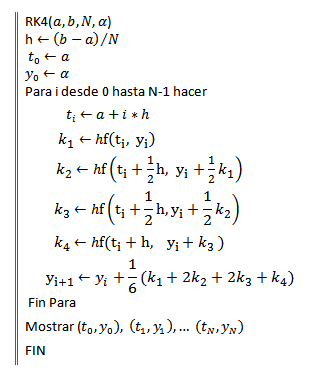
\includegraphics[width=0.50\textwidth]{alg_rk4}
%\caption{Figura-I.\label{fig: tahi}}
%}
%\end{figure}

.
\begin{definition}

\end{definition}

\begin{theorem}

\end{theorem}

\begin{corollary}

\end{corollary}

.



{\footnotesize
\begin{hangref}
\item Banks, J., J. S. Carson, B. L. Nelson, and D. M. Nicol. 2000. \textit{Discrete-Event System Simulation}. 3rd ed. Upper Saddle River, New Jersey: Prentice-Hall, Inc.
\end{hangref}
}




\bibliographystyle{wsc}
\bibliography{demobib}




\section*{Agradciemientos}


\appendix

\section{Anexos} \label{app:quadratic}

\begin{equation} \label{eq:quadraticsol}
x = \frac{-b \pm \sqrt{b^2-4ac}}{2a} \mbox{ si } a \ne 0.
\end{equation}


\end{document}

